% TODO rename Introduction and Background ?
\chapter{Introduction and Background}

[tbd]

\begin{itemize}
	\item Explain structure and main goal of this thesis
	\item Describe shortly all sections from this chapter and what the reader can expect
	\item Give short outlook to following chapter
\end{itemize}


%TODO
% internet schreibweise: Gross oder kleines I
% when to use italic for a term and when not ?
% numbers: 1´000 or 1,000 or 1000 ? 12.3 or 12,3 ?
% for example: e.g., i.e., "for example" .. ?


% ---------------------------------------------------------------------------------------------------------
% ---------------------------------------------------------------------------------------------------------


\section{E-Commerce}
\label{chapter:e-commerce}

This chapter gives an introduction to e-commerce.
Before going into the details, the emergence of e-commerce is described, starting with the Internet in section \ref{chapter:internet}.
In the following, I will briefly discuss the history of e-commerce and its types in section \ref{chapter:ecommerce_subchapter}.
The relationship between user satisfaction and the website performance is covered in section \ref{chapter:user_satisfaction}, which then leads to the chapter \ref{chapter:web_analytics} which is about web analytics.



\subsection{The Internet}
\label{chapter:internet}

In the last 50 years, a new technology emerged, spread over the entire world and influenced many aspects of most peoples life.
Within the turmoil of the cold war, the United State's \textit{Advanced Research Projects Agency} (ARPA) established in 1957 a communication network to bring together universities and their researches all around the country in order to be able compete against the USSR \cite{2011Cohen}.
What started as a tool for scientific collaboration evolved half a century later into the \textit{Internet}, a global network and phenomenon, to which every user with a dedicated device has access and can contribute to.
The internet is an integral part, if not the backbone of today's everyday life.
Users of the internet use it for almost everything, from sending emails, watching television, chatting with friends,  order lunch, checking the weather for the next day or renting motorized scooters.

% [Numbers]
In 2021, the internet has 4.66 billion users, which is around 60\% of the world population.\footnote{Following statistics are taken from \url{https://datareportal.com/reports/digital-2021-germany} [14.05.2021]}
Compared to 2020, the number of internet users increased by 7.3\%.
In Europe, more than 90\% of the population are internet users.
For a developed country like Germany, the numbers are even more impressing:
94\% of the German population are using the internet with an average daily time of over five hours.

Those numbers demonstrate impressive that the internet is an integral part of our daily life.
Along the rise of the internet, transactions and processes falling under the term of e-commerce are climbing as well.
Before discussing the term "e-commerce" and take a grasp at its history and types, some statistics are presented to demonstrate the importance of e-commerce.


\subsection{E-Commerce}
\label{chapter:ecommerce_subchapter}


\subsubsection{Introduction}

From the global data report\footnote{\url{https://datareportal.com/reports/digital-2021-germany} [14.05.2021]}, one can read out that over 90\% of the world population visited an online retail site and over 76\% of the world population purchased a product online.
% For most of the categories growth is over 15\%.  %TODO which categories ?
As usual, for or a western country like Germany, the figures are higher:
92.5\% of the German population visited an online retail site and over 80\% purchased a product online.
And the usage is expanding: the growth of the amount spent within the category food and personal care is 28.6\%, and 17.6\% for the category fashion and beauty.

E-commerce sales have grown steadily over the past 20 years, topping to 57.8 billion in 2019.\footnote{\url{https://einzelhandel.de/presse/zahlenfaktengrafiken/861-online-handel/1889-e-commerce-umsaetze} [14.05.2021]}

% [Corona: Even more growth]
The COVID-19 pandemic with its implications had and still has an not negligible impact on the growth of e-commerce.
Several measures were taken to stop the spread of the virus and the number of deaths, one of which was to minimize physical interaction between people.
This leads consequently to a shift of human interactions to the internet.
Along this, e-commerce benefits.
Bhatti et al. \cite{2020Bhatti} conclude that "e-commerce enhanced by COVID-19".



\subsubsection{Brief History}

E-Commerce, or electronic commerce, is according to the \textit{Encyclopædia Britannica} about "maintaining relationships and conducting business transactions that include selling information, services, and goods by means of computer telecommunications networks."\footnote{\url{https://www.britannica.com/technology/e-commerce} [19.05.2021]}
In short, e-commerce is about buying and selling products and services via the internet.

%TODO check for Tian when paper available:

The success of e-commerce is closely linked to the tremendous advances in Internet technology in recent years:
The development of the \textit{Electronic Data Interchange} (EDI) starting in the 1960s standardised the communication between two machines.
Personal computers were introduced in the 1980s, and one of the first examples of an online shop is the \textit{Electronic Mall} opened by CompuServe in 1984.
Another crucial milestone is the launch of the \textit{World Wide Web} (WWW) in 1990, which made the internet accessible to everyone.
With social media visible on the horizon from the 2000s, new possibilities for businesses and consumers alike to participate in e-commerce arise, for example, by enabling new marketing strategies or providing new sales channels.
New devices such as smart phones and tablets lowered the barrier to participate in e-commerce.
While e-commerce was available at any time, the new devices brought flexibility and mobility, making e-commerce available everywhere \cite{2019Hermogeno}.

With the continued advancement in technology, e-commerce can expect a bright future with trends such as AI recommendation systems, outstanding UX thanks to virtual reality, or even more simpler payment methods through cryptocurrencies.\footnote{\url{https://www.spiralytics.com/blog/past-present-future-ecommerce/} [19.05.2021]}



\subsubsection{Types}

There are several types in e-commerce and they emerge from the possible combinations between the actors \textit{business}, \textit{consumer} and \textit{government} \cite{2017DosSantos}.

\begin{table}[h]
	\centering
	\begin{tabular}{| c | c | c | c |}
	\hline
	 & Business & Consumer & Government \\
	\hline
	Business & B2B & B2C & B2G \\
	\hline
	Consumer & \cellcolor{lightgrey} & C2C & C2G \\
	\hline
	Government & \cellcolor{lightgrey} & \cellcolor{lightgrey} & G2G \\
	\hline
	\end{tabular}
	\caption{\label{tab:table-name} Types of e-commerce.}
\end{table}


\paragraph{B2C}
Business to Consumer in e-commerce describes basically online shopping, by means of a business offering its services and products to the consumer over the \textit{WWW}.
The consumer can browse through the products and services presented within an online shop and order them directly via the website.
A variety of payment and delivery options conclude the B2C type \cite{2020Heinemann}.
% TODO cite Heinemann with correct page p. 75 ?

%TODO where to put this sentence?
For an aspiring business, there are several ready-made software solutions for setting up an online store, as for example. \textit{Shopify}, \textit{ePages}, \textit{Magento} or \textit{WooCommerce} \cite{2019Steireif}.

A famous example of a B2C company is \textit{Amazon}.
On the 16th of July in 1995, Amazon launched as a website and entered the stock market on the 15th of May 1997 \cite{2019Stone}. % cite also that this is directly from page p. 47 ?
Amazon has been successful, with the stock starting at \$1.5, which is at around \$3200 as of this writing.\footnote{\url{https://finance.yahoo.com/quote/AMZN?p=AMZN} [19.05.2021]}
Today, Amazon employs over 1 million people\footnote{\url{https://www.statista.com/statistics/234488/number-of-amazon-employees/} [19.05.2021]} and serves the desires of 200 million paying prime members.\footnote{\url{https://www.statista.com/statistics/829113/number-of-paying-amazon-prime-members/} [20.05.2021]}
\\

% [Pro and Con]
By taking a quick look at the pros and cons of an online store, it becomes clear that some of the advantages are that: there is no need of a real, physical store to showcase and sell the products; the virtual shop is available to the consumer at any time and has no closing hours; there is a high potential for the online shop as it is part of growing market; online business is scalable; due to tracking algorithms, precise targeting as well as data analysis is possible; to start an online business, there is not so much floating required and there are generally lower costs; it is possible to provide a personalized customer experience.

Some disadvantages are that the speed of market is rapid, competitors arise everyday everywhere and technology evolves quickly while consumers expectations go high \cite{2019Hermogeno}, \cite{2020Lang}.
\\

% [Performance of online shop is important]
Another disadvantage is that there is no direct or physical connection with the consumer.
As described above, online shopping takes place on the virtual WWW, i.e. personal interaction between buyer and seller is not possible and the shopping experience takes place on a website, from which it follows that the overall virtual user experience must be excellent in order to compete.

In the next section, I will describe the findings between the correlation between user satisfaction and the performance of the retailers web presence.



% ------------------------------------------


\subsection{User Satisfaction and Performance}
\label{chapter:user_satisfaction}

% [User Satisfaction]
The aim of this thesis is not to deep dive into terms and concepts or the non-trivial problem of defining user satisfaction, usability or the like.
Therefore the term user satisfaction is in this context loosely defined as how happy the user is with the website he or she interacts with.\footnote{For a discussion cf. "User satisfaction measurement" in \cite{2010Islam}}

% [Performance]
Performance can be understood as the speed of an online shop, e.g. how long it takes the page to load, how quickly the user can interact with the page, and how the user perceives the performance of the website.
In chapter X I will discuss that measuring performance is not so trivial and there are a lot of ideas and metrics to measure it. %TODO in chapter X


% [SpeedHub]
\subsubsection{SpeedHub}

A plethora of information and studies about the phenomenon of user satisfaction and web site performance is collected at \textit{SpeedHub.org}, a portal by \textit{Baqend} in cooperation with \textit{Google} which provides "the largest systematic study of Mobile Site Speed and the Impact on E-Commerce."\footnote{\url{https://www.speedhub.org/} [21.05.2021]}
Not only are studies and reports available on the hub, but also collections of videos and blog posts.

% [code.talks 2019]
In his talk at code.talks 2019, Felix Gessert summarizes the results and provides insights into the most important aspects and questions of the study so far \cite{2019Gessert}:

% [User Profile and Psychology]
The first observation when asking for a correlation between the performance of a system and user satisfaction is that users need to be differentiated, which leads to the concept of a \textit{User Profile}: In terms of gender, young women are the most demanding consumers and are less likely to buy from slow sites.
In general, people between the ages of 18 and 24 have higher expectations of a site's speed than their older counterparts.

There are also differences between nations and regions, for example people from Japan have the highest expectations, which is almost certainly related to technological advancements in that country.
Not only the expectations themselves differ geographically, but also how speed influences the users, for example "speed influences New Yorkers more than Californians." \cite{2019Thinkfast}, \cite{2017Brainfood}

What all users have in common is their human psychology. 
In terms of performance, researchers generally suggest keeping wait times below one second to keep users' attention. (cf. "Performance perception" in \ref{chapter:web_performance}). 

% [Devices]
After considering the user himself, the next step is to examine the influence of the device used: Studies show that mobile users are more likely to buy products and services than their colleagues using a desktop computer, where iOS users have generally more expectations regarding site speed \cite{2019Deviceatlas}.
 
% [Context]
Last but not least, the context and state of the user is important, with naturally relaxed and calm users perceiving pages faster than stressed or hurried users.
Also users experience websites more slowly while on the go \cite{2014Akamai}.
\\

% [Studies]
There are many real world examples and studies that prove and demonstrate the importance of website speed in terms of user satisfaction and ultimately sales:
\textit{Amazon} found out that a decrease of 100 ms in page loading leads to -1\% conversion rates.
If the site loads 100 ms faster, \textit{Walmart} observed that the revenue increases by 1\%.
For \textit{Zalando}, increasing site speed by 100 ms has led to an uplift of 0.7\% revenue per session \cite{2006Linden}, \cite{2018Zalando}, \cite{2012Walmart}.


% [SEO]
Search engine optimization is heavily impacted by load speed:
For \textit{Google}, 500 ms slower sites led to a decrease of 20\% in traffic.
\textit{GQs} traffic increased by 80\% after the page load went down from 7 s to 2 s.
And for \textit{Pinterest}, 40\% faster loads led to 15\% more SEO traffic \cite{2015GQ}, \cite{2006Mayer}, \cite{2017Pinterest}.


% [Engagement & Satisfaction]
User engagement and satisfaction also depend heavily on loading times:
\textit{Forrester} noted an increase of 60\% for the session length while brining down the load time by 80\%.
\textit{Akamai} monitored that the bounce rate climbed up incredible 103\% when the load time increased by 2 seconds.
And for the \textit{AberdeedGroup}, the customer satisfaction dropped by 16\% at one more second delay in response times \cite{2017Forrester}, \cite{2017Akamai}, \cite{2008Aberdeen}.

In summary, it can be said that many studies and practical examples prove and demonstrate that faster websites and online stores lead to a better user experience and usually to happier customers.
In commercial terms, one can conclude that page speed equals money.
\\

In order to properly test the effects of performance on users, a scientific method is required.
A/B testing as a controlled experiment is one of them and will be explained in the next section.
After discussing A/B testing, I will move on to examining \textit{Web Analytics}, a term that encompasses methods, tools, and instruments for companies to better understand their business and customers.


\subsubsection{A/B Testing}

Controlled experiments like A/B testing are not a new tool for scientists and researchers and were used as early as the 1920s \cite{2016Kohavi}.
With the advent of the Internet in the 1990s, the concept was adopted into the online domain and is now used by large companies such as Amazon, Facebook or Google to test ideas and hypotheses directly on a live system.
Controlled experiments such as A/B testing are used to aid decision making and provide a "causal relationship with high probability" \cite{2016Kohavi}.
They enable a data-driven and quantitative validation of the hypothesis \cite{2018Morys}.

Controlled experiments help to test hypothesis and questions of form: "If I change feature X, will it help to improve the key performance indicator Y?"

To answer this question,  two systems are needed: \textit{Version A}, the control variant or default version, and a slightly different \textit{Version B,} called the treatment.
If more than two versions or one treatment should be evaluated at the same time,  an A/B/n split test has to be implemented.
With a univariable setup, only one variable differs between the systems; with a multivariable structure, several variables are changed at the same time.

Usually, the users of the system are randomly split into two groups and testing is directly performed with real users on a production system.
It is advantageous, also compared to other experimental set-ups, that the users and participants are not aware that they are part of an experiment, which leads to fewer biases and side effects.
In order to measure the differences and the user behaviour, web analytics has to be integrated within the system \cite{2016Kohavi}.

A brief and general discussion of controlled experiments in computer science can be found in chapter X.  %TODO link chapter about controlled experiments
\\

% [Transition to Web Analytics]
To continue with the question of performance and user satisfaction, A/B testing allows two different versions of the same site to be served to two groups at the same time, one site being slow and the other being fast, without users knowing.

An implemented web analytics system makes it possible to measure how the various systems and user groups behave.
What web analytics exactly is, what tools are available and what a web analytics process looks like, is discussed in the next section.



% TODO write those steps down ?
% 2018 Morys
%- 5 steps:
%- 1. quality of hypothesis according to SOR Paradigma
%- 2. quality of testconcept: isolation and contrast of changed parameters
%- 3. quality of implementation and quality assurance: running tests should not be visible by user (e.g. suddenly UI changes) and performance of website should not be impacted
%- 4. quality of measurement: significant difference in primary goals
%- 5. quality of statistical interpretation: amount of data, statistical methods

% 2012 Kessler 17.2  AB Tests ?
% Heinemann 2020 A/B Tests nach 4.1.4 ?



% ------------------------------------------------------------------------------------
% ------------------------------------------------------------------------------------
% ------------------------------------------------------------------------------------
% ------------------------------------------------------------------------------------



\section{Web Analytics}
\label{chapter:web_analytics}

This chapter is about web analytics.
I will first discuss definitions and give a short introduction to web analytics in section \ref{chapter:web_analytics_introduction}.
Then, a brief history of web analytics will be given in section \ref{chapter:web_analytics_history} to help contextualize.
After characterizing two web analytics process descriptions in section \ref{chapter:web_analytics_process}, data collection methods will be discussed in section \ref{chapter:web_analytics_logfile_pagetagging}.
Finally, web performance will be explained in \ref{chapter:web_performance}, which leads the way to the research questions.


\subsection{Introduction}
\label{chapter:web_analytics_introduction}

% [Definitions]
What is \textit{Web Analytics}?
Reviewing the literature, it is clear that there are several definitions:

Nakatani et al. state that "Web analytics is used to understand online customers and their behaviors, design actions influential to them, and ultimately foster behaviors beneficial to the business and achieve the organization's goal." \cite{2011Nakatani}
According to this definition, web analytics is about getting insights of the users using the system, not only who or what they are, but also how they interact with the system.
Additionally, the definition emphasizes that the underlying motivation of web analytics is to achieve business goals.

Singal et al. provide a more technical definition by pointing out that "Web Analytics is the objective tracking, collection, measurement, reporting and analysis of quantitative internet data to optimize websites and web marketing initiatives." \cite{2014Singal} %TODO note that this definition is directly taken from Kaushik ?
Again, the ultimate goal is to drive business, but supported by data science methods and tools such as tracking, collecting and analysing massive amounts of data.

Bekavac et al. provide a similar definition by pointing out that web analytics is "the analysis of qualitative and quantitative data on the website in order to continuously improve the online experience of visitors, which leads to more efficient and effective realization of the company's planned goals." \cite{2015Bekavac}

% TODO: where can i find this officially ?
% Official definition by WAA: the measurement, collection, analysis and reporting of Internet data for the purposes of understanding and optimizing Web usage.

% TODO add 2009 Waisberg? "Web Analytics can be defined as the act of increasing a website’s persuasion and relevancy to achieve higher conversion rates."

% TODO add Croll 2009? "Today, web analytics is a marketing discipline used to measure the effectiveness of communications strategies" p.83

Summarizing the above definitions, it is noticeable that web analytics consists of two important elements: a data-driven, information-oriented and technical element of collecting and analysing data about users and a commercial and business-driven element that provides the main motivation for collecting the data primarily by setting business goals.
\\

% [Use Cases]
Moving from definitions to the practical realm, Zheng et al. describe four main use cases for web analytics \cite{2015Zheng}:

\begin{itemize}
\item Improving the overall design and usability, for example of the navigation or layout of the website.
\item Optimize for your business goals: Whatever goals the business is trying to achieve, generating conversions is the goal.
\item Monitor campaigns: Understand and measure the success of advertising campaigns.
\item Improve performance by examining metrics such as page load time. This is discussed further in chapter \ref{chapter:web_performance}.
\end{itemize}

% [Challenges]
Web analytics is also difficult and there are some obstacles and challenges to overcome.
Kumar et al. describe some of the hurdles as follows \cite{2019Kumar}:
The analysis and interpretation of the data and the goals and measures derived from it are reactive rather than anticipatory, since "predictive modelling applications" for web analytics are not yet on the market.

Big data, that is the volume, variety and velocity of data collected, can be challenging to manage,
for example, important insights can be lost or overlooked.

Privacy and the information collected from visitors and customers can be another challenge in terms of inappropriate use of data and GDPR compliance.



% ------------------------------------------


\subsection{Brief History}
\label{chapter:web_analytics_history}

The history of web analytics can be described as a transformation from an IT domain and a technical log file analysis tool to a sophisticated, polymorphic tool for marketers.

% [For IT: Logs]
Each time a user requests an HTML file or other resource from a web server, the server makes an entry in a special log file \cite{2014Singal}.
The first log entries followed the \textit{Common Log Format} (CLF) which provides rudimentary information such as the date, the HTTP status code or the number of bytes transmitted.
In 1996, the \textit{Extended Log Format} (ELF) was introduced with more flexibility and information in mind.
Thanks to the standardized format of the log files, it was possible to create software that evaluates the log files and presents them to users in a readable form.
\textit{GetStats} was one of the first tools which generated statistics and user friendly output for analysts \cite{2009Croll}. %TODO add p. 69?
In 1995, Dr. Stephen Turner developed \textit{Analog}, the first free software for analysing log files \cite{2015Zheng}.
Log file analysis will be further discussed in chapter \ref{chapter:log_file}.

% [Shift]
What was initially mainly interesting for maintenance and IT staff, who for example answered the question of how many 404s occurred on the server, developed into an interesting website information pool for marketers.

As the available information increased, it became clear that the data could be used for more than just analyzing server behavior.
But log file analysis was not enough to provide details about how users interact with the site.
Web analytics underwent a transformation from log analysis to user data tracking, analysis, and reporting.

Croll describes the move of analytics from IT to marketing with three steps: \cite{2009Croll}
\begin{enumerate}
\item JavaScript eliminated the need for log files and enabled marketers to maintain and deploy their analytics solutions themselves, making them less dependent on IT.
\item The introduced advertising economy of search engines like Google led to a new focus of analysts on user attraction and conversion rates.
\item New cost models allowed marketers to pay for the analytics service based on website traffic, rather than paying upfront for hardware and software. Analytics spend was thus linked to website traffic and, ideally, revenue.
\end{enumerate}

% [For Marketing: JS]
In 1990 the WWW started and in 1993 one of the first widely used browsers \textit{Mosaic} was launched.
At the same time \textit{WebTrends} developed and released one of the first analytics software.
A lot more services followed, such as \textit{WebSideStory} in 1996 \cite{2009Croll}
or \textit{Quantified} by Urchin in the same year \cite{2009Croll}.

Page tagging made it possible to collect not only technical data, but also business-relevant information.
Visitors and their behaviour were the focus, shaping questions like: How is this user behaviour related to a purchase? If a user buys shoes, will he also buy socks?
The development and implementation of cookies enabled the identification of unique users.
Not only business-relevant questions were asked and answered, but also studies on performance and usability \cite{2009Croll}. %TODO add p. 69 ?
More details about page tagging can be found in chapter \ref{chapter:page_tagging}.
\\

% [WAA, Today]
In 2003, Edwards, Eisenberg and Sterne founded the \textit{Web Analytics Association} (WAA).
The WAA brings together and supports all the players in web analytics such as users, marketers and IT specialists on an international stage.
Due to digitalization and its all-encompassing effects, the WAA has renamed itself \textit{Digital Analytics Association} (DAA) in 2012 because the web is not the only area where users leave their digital footprint \cite{2014Singal}.
%TODO rewrite above sentence

As described in the section above, participant and user numbers on the Internet continue to rise and now all Fortune 500 companies operate websites, with web analytics a key marketing tool \cite{2019Kumar}.

Some of the most established tools today are \textit{Google Analytics}, \textit{Adobe SiteCatalyst}, \textit{Webtrekk} and \textit{Piwik} \cite{2020Heinemann}. %TODO add chapter 4.1.4
Google Analytics will be further discussed in chapter \ref{??}. %TODO add reference

% [Future]
Looking ahead, Zheng et al. identify several trends for web analytics, such as mobile web and application-specific analytics like video, search, learning, or social media analytics \cite{2015Zheng}.


% TODO next section will be about process ??

% TODO add Image: Genesis of Web Analytics (nice graphic) with WAA, DAA ? should remove then in-page analytics arrow

% TODO add somewhere Some methods about tool selection are described in chapter X.


% ------------------------------------------


\subsection{Web Analytics Process}
\label{chapter:web_analytics_process}


Web analytics can be described as a process in which the main goal is usually to increase sales.
The literature cites two main ideas and processes, the first from the Web Analytics Association and the second from industry best practices.
They are briefly described in this section.

Both processes have in common that they are aimed at improving the website and thus increasing business revenue.

% [KPIs]
\textit{Key Performance Indicators} (KPIs) are the ideal tool for the instrumentation of web analytics and help to identify areas and potential for improvement.
They are an integral part and play an important role in any web analytics process as they provide a "in-depth picture of visitor behavior on a site" \cite{2009Jansen}. %TODO add ch. 6.2 ?

KPIs can differ depending on the business in which they operate.
For commercial domains, common KPIs are conversion rates, average order or visit value, customer loyalty, bounce rate, etc. \cite{2014Singal}.

Defining the right KPIs and aligning them with business goals is a critical step in any web analytics process.

% TODO add more ?:
% 2015 Bekavac:  KPIs for commercial model: Ratio of new to returning visitors, percentage of new visitors, referring domains, search keywords/phrases, average order value, key conversion rates



\subsubsection{WAA Process Guide}

% TODO compare both processes directly with a table with 2 columns?

The Web Analytics Association offers a web analytics guide that consists of nine steps. They are: \cite{2009Jansen} %TODO add ch. 6.2 ?

\begin{enumerate}
\item Identify key stake holders
\item Define primary goals of website and prioritize them
\item Identify most important site visitors
\item Determine key performance indicators
\item Identify and implement the right solution
\item Use multiple technologies and methods
\item Make improvements iteratively
\item Hire and empower a full-time analyst
\item Establish a process of continuous improvement
\end{enumerate}


\subsubsection{Industries Best Practices}

On the contrary, Waisberg and Kaushik derive a five-step process from industry best practices with the main goal of improving the website and increasing sales \cite{2009Waisberg}: %TODO improve waisberg citation

\begin{itemize}
\item Define Goals
\item Build KPIs
\item Collect Data
\item Analyse Data
\item Implement Changes
\item Repeat last two steps
\end{itemize}

% TODO add graphic instead of list ??


% [Comparison]
When comparing the two proposed processes, it becomes clear that both focus on identifying and being aware of the most important business goals.
The WAA process is a finer-grained and more practical approach, with Waisberg and Kaushik abstracting the main activities.



% ------------------------------------------



\subsection{Log File Analysis and Page Tagging}
\label{chapter:web_analytics_logfile_pagetagging}

There are four main methods of collecting data for web analytics: through log file analysis, JavaScript page tagging, web beacons, and packet sniffing \cite{2009Waisberg}.

As already mentioned in chapter \ref{chapter:web_analytics_history},  the two most important methods of data collection are log file analysis and page tagging.
In this section I will briefly describe and compare both mechanisms.



\subsubsection{Log File Analysis}
\label{chapter:log_file}


As already described, the log file analysis is about gaining knowledge from the log file records of the web server.
Log file analysis is considered to be the traditional and original approach to web analytics \cite{2011Marek}, \cite{2015Zheng}. %TODO improve Marek citation
As soon as the user types a URL into the browser and presses the enter key, the request arrives at a web server.
The server then creates an entry in a log file and sends the requested page or resource back to the client in response \cite{2009Waisberg}.
The information within the log entry can vary depending on the log format, usually IP, browser, time stamp, time required, transferred bytes, whether a cache hit occurs and the referrer is specified \cite{2009Waisberg}.
The standardized Common Log Format provides host, ident, authuser, date, request, status, bytes, as can be seen in listing \ref{lst:log}.\footnote{\url{https://www.w3.org/Daemon/User/Config/Logging.html\#common-logfile-format} [03.06.2021]}

\begin{center}
\begin{lstlisting}[caption={CLF}, language=bash, numbers=none, basicstyle=\tiny, label={lst:log}]
127.0.0.1 user-identifier frank [10/Oct/2000:13:55:36 -0700] "GET /apache_pb.gif HTTP/1.0" 200 2326
\end{lstlisting}
\end{center}
% TODO add caption

Standard formats of log files and entries enable log file analysis software to process, evaluate and report valuable statistics such as \textit{Analog}, \textit{Webalizer} or \textit{AWStats} to users \cite{2015Zheng}.


% [Pro]
Below are a few points that describe the pros and cons of log file analysis.
The advantages of log file analysis are (\cite{2009Waisberg}, \cite{2011Nakatani}, \cite{2014Singal}, \cite{2015Zheng}):
%TODO just cite here above all or in the list ?

\begin{itemize}
\item JavaScript and cookies are not required on the client side
\item Maintainer of the website and server owns the data %cite 2009 Waisberg
\item Bots and web crawler requests are also logged %cite 2009 Waisberg
\item History of data is available %cite 2011 Nakatani
\item Log entries are reliable %cite 2011 Nakatani
\item The standard format of log files enables easy switching of analysis tools %cite 2011 Nakatani
\item The web server also logs failed requests %cite 2011 Nakatani
\item No modification on the web page needed %cite 2015 Zheng
\item Does not demand more bandwidth %cite 2014 Singal
\end{itemize}


% [Con]
Some disadvantages of log file analysis are (\cite{2011Marek}, \cite{2015Zheng}):

\begin{itemize}
\item Log entries provide mainly technical information, which may not be very useful for user behaviour analysis. Business related metrics such as bounce rates are not available. % cite Marek 2011
\item Only direct requests from the client to the web server are logged: Any user interaction in the web browser that does not trigger a request is not logged. Responses from caches and proxies are also not visible in the web server's log file. Only interactions with the web server are logged.
%cite 2015 Zheng
\end{itemize}



% ------------------------------------------


\subsubsection{Page Tagging}
\label{chapter:page_tagging}

In a nutshell, page tagging describes the analysis method used to incorporate JavaScript into the website, which collects data and sends it to an analysis server \cite{2011Marek}.
To do this, JavaScript must be integrated on every page to be analysed \cite{2009Waisberg}.
Page tagging is the most important method in web analytics today \cite{2015Zheng}.


Croll provides a illustration (figure \ref{img:page_tagging}) of the page tagging process which is explained below \cite{2009Croll}.

\begin{figure}[h!]
\begin{center}
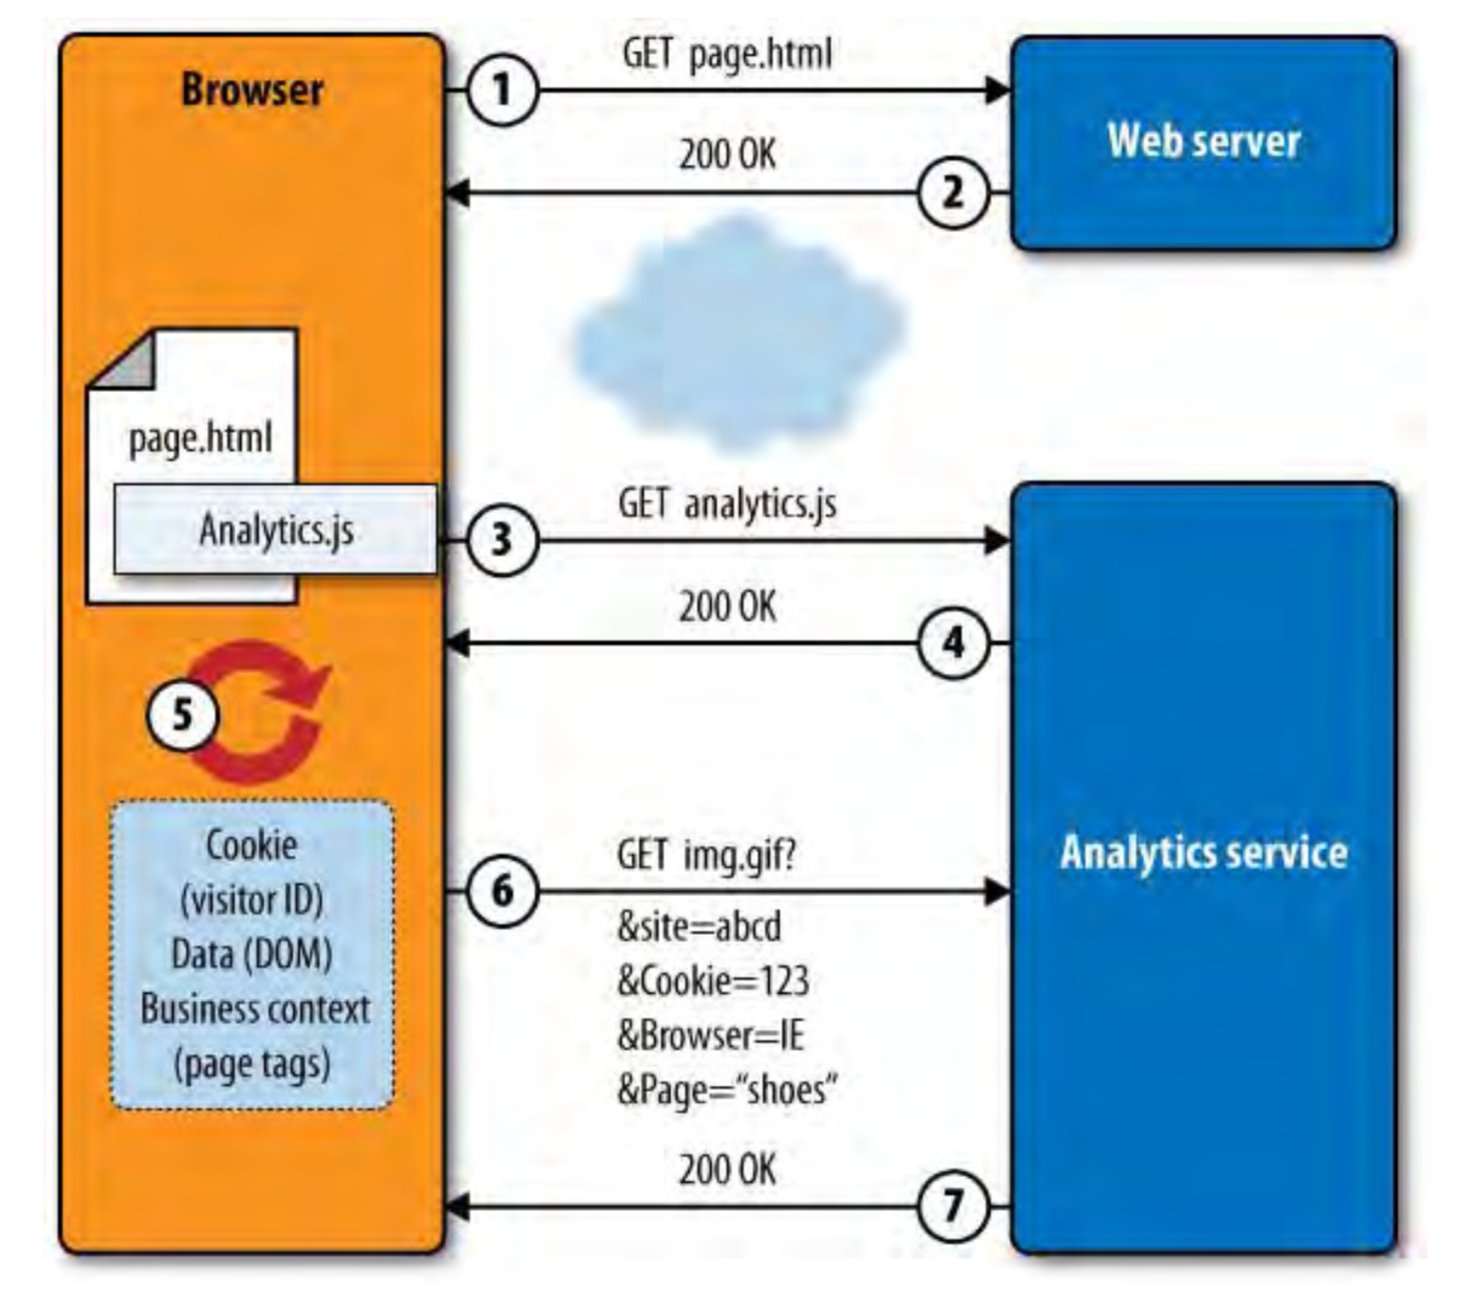
\includegraphics[width=0.5\textwidth]{page_tagging.png}
\caption{Page Tagging}
\label{img:page_tagging}
\end{center}
\end{figure}

The client (browser) requests a page from the web server (1, 2).
Within the HTML file an external JavaScript resource, the analytics code, is linked and received from the analytics server (3, 4).
The analytics script tracks and measures the user behaviour and eventually sends the data back to the analytics server (5, 6, 7).

The data collected can also be stored in cookies, which contain data beyond a session and enable the user to be identified, e.g. the next time he visits the page \cite{2019Kumar}.


The advantages and disadvantages of page tagging are as follows, starting with the pros (\cite{2009Waisberg}, \cite{2011Nakatani}, \cite{2011Marek}, \cite{2014Singal}, \cite{2015Zheng}):

%TODO again put all references on top ?

% [Pro]
\begin{itemize}
\item Every page visit is counted %cite 2009 Waisberg
\item The analytics service is outsourced, which includes the storage of the data, but also the data analysis and reporting %cite 2009 Waisberg
\item Page tagging is rather easy to implement and favourable when the analyst does not have access to the web server %cite 2011 Marek
\item Highly customizable: Everything that JavaScript enables to measure, collect, and track is available. This also includes information about the client such as screen size, device used or color depth. %cite 2011 Nakatani
\item Ability to track events and actions such as mouse clicks that do not send requests to the web server. This is especially important for single-page or progressive web applications that do not generate requests as often.  %cite 2011 Nakatani and 2015 Zheng
\item Mechanics of cookies provide identification of unique and repeat visitors %cite 2011 Nakatani
\item Real time reporting is possible %cite  2014 Singal 
\end{itemize}


% [Con]
Some drawbacks are mainly privacy concerns, that the analysis process relies on the use of JavaScript and cookies that can be disabled by the user \cite{2011Marek}, that every page that is supposed to collect data must contain the analytics script and due to the use of a third party analytics service it is pretty difficult to switch tools \cite{2014Singal}.

% TODO 2017 Hassler ch. 2 ??

% TODO web beacons and packet sniffig ?:
% 2011 Marek
% 2011 Nakatani
% 2014 Singal




% ------------------------------------------


\subsection{Web Performance}
\label{chapter:web_performance}

% [Introduction]
This chapter gives only a brief overview of the various aspects of web performance.
Reference is made below to the appropriate sections that cover the topics in more detail.

% [Definitions]
As already described in chapter \ref{chapter:user_satisfaction}, web performance plays a role that cannot be neglected for user satisfaction and business success.
The above studies show that increasing website performance also increases sales, or as Google states it: "Performance plays a major role in the success of any online venture".\footnote{\url{https://web.dev/why-speed-matters/} [03.06.2021]}

The MDN Web Docs identify multiple areas of web performance:\footnote{\url{https://developer.mozilla.org/en-US/docs/Learn/Performance/What_is_web_performance} [03.06.2021]}
\begin{itemize}
\item Reducing overall load time
\item Making the site usable as soon as possible
\item Smoothness and interactivity
\item Perceived performance
\item Performance measurements
\end{itemize}

%TODO add chapter references
\paragraph{Reducing load time}

The question of what makes websites slow is covered in chapter X.


\paragraph{Usability and interactivity}

As I will describe in chapter X, there are several metrics available that attempt to reflect areas of performance such as load time, smoothness, and interactivity, and specific metrics are available as well as for differentiating between technical and user-perceived performance.


\paragraph{Performance perception}

The perception of performance is generally subjective.
As already seen in chapter \ref{chapter:user_satisfaction}, there are some quantifiable time intervals that correlate with human psychology regarding the received performance.
Table \ref{table:perception} contains "unofficial rule of thumb" for delay thresholds \cite{2013Grigorik}.


\begin{table}[h]
	\centering
	\begin{tabular}{| l | l | }
	\hline
	Delay & User Perception \\
	\hline
	0-100 ms & Instant \\
	100-300 ms & Small perceptible delay \\
	300-1000 ms & Machine is working \\
	> 1 s & Likely mental context switch \\
	> 10 s & Task is abandoned \\
	\hline
	\end{tabular}
	\label{table:perception}
	\caption{Rule of thumbs for delay}
\end{table}

If one interprets the numbers from the table, one can make the statement that it is desirable to keep loading times below one second.
Thresholds for certain performance metrics and the psychological rationale for setting them are discussed in chapter X. %TODO


% TODO add this?
% https://developer.mozilla.org/en-US/docs/Learn/Performance/why_web_performance
% financial aspect of downloading data and big websites



\paragraph{Performance measurements}
%TODO

There are several methods of measuring performance.
\textit{Synthetic monitoring }is discussed in chapter X.
\textit{Real User Monitoring} (RUM) is covered in chapter X.





% ---------------------------------------------------------------------------------------------------------------------------------
% ---------------------------------------------------------------------------------------------------------------------------------


\section{Research Question}
\label{chapter:research_question}

The e-commerce industry is booming and there are no signs that this trend is reversing; on the other hand.
Performance plays an important role in terms of customer satisfaction and how this directly affects business revenue.
To better understand e-commerce website visitors, page tagging is widely used and implemented.

Several questions and issues can arise in this area and context, such as: Does page tagging affect the website's performance?
Intuitively, it can be said that loading additional JavaScript will reduce the performance of the website, depending on parameters such as the script size and network condition.
But are there more unpredictable side effects?
Do the various techniques of embedding a tracking script affect the data collected and measured?
Will the various tracking scripts supplied interfere with each other?

A hypothesis of this work is that tracking tools slow down the monitored websites, reduce the speed and performance of the website and thus have an unfavourable effect on the user experience.

These questions are to be investigated within the scope of this thesis.


\subsection{Goal}

This thesis has several goals:

The Internet and websites in general are complicated, complex, and tangled.
Although basic HTML structures are standardized, each website follows its own form and is unique and sui generis.
In order to conduct a controlled experiment and test hypotheses, one goal is to approximate real websites with an artificial, laboratory-generated website that is completely controlled and manipulated by the researcher.

The aim is to create a reliable, but also convincing test environment in order to model and reproduce real behaviour.

Once the test environment is up and running, performance measurement issues need to be addressed.
The aim is to measure, collect, visualize and analyse performance data.

As we will see in chapter X, there are many metrics for measuring performance.
Another goal of this work is to establish something like a taxonomy of performance metrics.





% The research motivation is to investigate if, and how tracking tools are slowing down websites and which particular features of those tools impact how and why the websites performance.

% Within this investigation, the trade-off between “meaningful” collected data and the websites performance is of special interest. The assumption is that slim, performant tracking tools may not aggregate that much useful data as heavy and presumably the website decelerating tools.



\subsection{Chapter Outline}

[tbd]

% TODO move this to beginning of introduction ?

Chapter 1 was about...
In Chapter 2 we see,
Chatper 3...













